\documentclass[fleqn,10pt]{wlpeerj}
\title{Large, structurally-curated alignment and phylogeny of Vertebrate biogenic amine receptors}

\author[1,2,3]{Stephanie J. Spielman}
\author[4,5]{Ahmad R. Sedaghat}
\author[1,2,3]{Keerthana Kumar}
\author[1,2,3]{Claus O. Wilke}
\affil[1]{Department of Integrative Biology, The University of Texas at Austin, Austin, U.S.A.}
\affil[2]{Institute of Cellular and Molecular Biology, The University of Texas at Austin, Austin, U.S.A.}
\affil[3]{Center for Computational Biology and Bioinformatics, The University of Texas at Austin, Austin, U.S.A.}
\affil[4]{Department of Otolaryngology–Head and Neck Surgery, Massachusetts Eye and Ear Infirmary, Boston, Massachusetts, U.S.A.}
\affil[5]{Department of Otology and Laryngology, Harvard Medical School, Boston, Massachusetts, U.S.A.}

\keywords{biogenic amine receptors, phylogenetics, multiple sequence alignment, G-protein coupled receptors}


\begin{abstract}


\end{abstract}

\begin{document}

\flushbottom
\maketitle
\thispagestyle{empty}


\section*{Introduction}

Biogenic amines, such as the molecules serotonin and dopamine, play critical roles in virtually all Metazoa taxa, exerting significant influence on both behavior and physiology particularly within the central nervous system. In Vertebrate species, their actions are mediated primarily through the biogenic amine receptor family, which includes dopamine (DRD), histamine (HRH), trace (TAAR), adrenergic (ADR), muscarinic cholinergic (mAChR), and most serotonin receptors (5HTR).  Biogenic amine receptors belong to the broad family of G protein-coupled receptors (GPCR), one of the largest and most diverse receptor families in eukaryota, and indeed Metazoa. Indeed, due to the extensive diversity of biological functions they direct and the ongoing expansion of their ligand repertoire, GPCRs are considered one of the most evolutionarily innovative and successful gene families \citep{BockaertPhillipe1999,Lagerstrom2008}.

Biogenic amine receptors fall in to the Rhodopsin-like (family ``A'') GPCR family, which emerged as a distinct GPCR clade with the origins of the Opisthokont (Fungi and Metazoa) lineage \citep{Krishnan2012}. Subsequently, the Rhodopsin-like family underwent substantial expansion in Metazoa, most notably in Vertebrate lineages \citep{Rompleretal2007,Staubert2013}. Like all GPCRs, these receptors are highly structurally conserved, containing seven transmembrane (TM) domains separated by three extracellular (ECL) and three intracellular (ICL) loops with an N-outside C-inside orientation, and they propagate intracellular signaling through a G protein-mediated pathway. Biogenic amine receptors are frequent targets for a wide array of pharmaceuticals aimed to treat diseases such as schizophrenia, migraines, hypertension, allergies and asthma, and stomach ulcers \citep{Schoneberg2004,Eversetal2005,Masonetal2012}.

In spite of these receptors' biological and clinical importance, studies on their evolution are relatively limited. Evolutionary studies which have focused on a biogenic amine receptors have predominantly been limited to single receptor subtypes, namely TAAR \citep{Gloriametal2005,Lindemann2005,Hashiguchi2007}, DRD \citep{Callieretal2003,Yamamotoetal2013}, and 5HTR \cite{Anbazhagan2010}. Moreover, many of these studies, and indeed larger-scale studies on the general evolution of the broad Rhodopsin-like GPCR family, have examined very narrow species distributions, for instance specifically teleosts \citep{Gloriametal2005}, primates \citep{Anbazhagan2010}, humans and mice \citep{Vassilatis2003,KakaralaJamil2014}, or even strictly humans \cite{Fredrikssonetal2003}. Therefore, studies which account for the full breadth of known bioamine receptor sequences as well as their broad species distributions 

This dearth of biogenic amine receptor-specific evolutionary understanding is underscored by the difficulties in establishing a robust multiple sequence alignment (MSA). Commonly used to identify conserved sequence motifs and functionally important residues as well as investigate the sequences' evolutionary history, MSAs provide the foundation for nearly all comparative sequence analyses. As MSA errors readily introduce bias these downstream analyses \citep{Ogden2006, Wong2008, Jordan2012}, it is crucial to ensure accuracy in the alignment to the extent possible. For GPCR sequences, in particular, any alignment should recapitulate their canonical 7TM structure, which a naive alignment of sequences cannot necessarily accomplish. While there are certain MSA software platforms which explicitly incorporate structural information into the alignment algorithm (e.g.\ 3DCoffe \citep{3dcoffee} and PROMALS3D \citep{promals3d}), these programs are fairly computationally-intensive and thus unwieldy (ill-suited?) for large-scale (over 1000 sequences) applications. Moreover, such programs require the use of a single crystal structure to guide sequence alignment. While all GPCRs have the same conserved 7TM domains, different GPCRs, and indeed the biogenic amine receptors, feature a wide variety of ICL and ECL sizes. For instance, the ECL3 lengths for human HRH1 and DRD3, respectively, are roughly 27 and 117, and their respective ICL3 lengths are 68 and 14 (as predicted by GPCRHMM \citep{Wistrand2006}). Thus, aligning with a single crystral structure will not effectively represent the domain variability across biogenic amine receptor subtypes. A desirable alignment strategy would ensure that all sequences are anchored by their conserved 7TM domains without inappropriately constraining the heterogeneous ECL and ICL domains.

We therefore have adopted a novel iterative alignment strategy to create a large (3064 sequences), structurally-curated MSA of vertebrate biogenic amine receptors. In order to ensure proper structural alignment, we employed the software GPCRHMM \citep{Wistrand2006}, which uses a hidden markov model approach to assign each residue in a given GPCR sequence to its respective domain, either extracellular, transmembrane, or intracellular. Previously validated with real GPCR crystal structures \citep{SpielmanWilke2013}, GPCRHMM relies on the remarkably-conserved GPCR 7TM structure to predict GPCR domains with exceptional accuracy and without the use of a crystal structure. Our alignment strategy therefore ensured that all predicted 7TM domains aligned appropriately across all sequences. Importantly, this strategy did not require any manual or visual data inspection, thus avoiding any confounding subjectivity in MSA processing. 

We present this biogenic amine receptor MSA as a resource for any group interested in studying the dynamic evolutionary processes, structural, and/or functional constraints operating on this exceptionally important GPCR clade. Moreover, to demonstrate the utility of our alignment, we constructed a phylogeny of our receptors with this alignment as well as a naive MSA which did not undergo this iterative process. We found that our structurally-curated MSA offered dramatic improvements over a structurally-naive MSA. Our structurally-aware MSA and corresponding phylogeny therefore represent the most comprehensive and curated vertebrate biogenic amine receptor dataset to date. Moreover, using this phylogeny, we are able to discern the relationships among receptor types with a far increased sensitivity than previous analyses. Even so, we are unable to fully resolve the deeper nodes in the phylogeny, revealing the capabilities and limitations of current-day phylogenetic methods.

\section*{Results}

\subsection*{Constructing a structurally-curated MSA of biogenic amine receptors}
We collected all sequences using PSI-BLAST and filtered data to ensure a high-quality data set (see \emph{Methods} for details). We additionally retained only sequences which the program GPCRHMM unequivocally classified as a true GPCR sequence, leaving a total dataset of 3464 receptor sequences to align. We then built a structurally-curated MSA from these 3464 receptor protein sequences according to the iterative strategy outlined in Figure~\ref{flowchart}. The resulting alignment, obtained after four iterations of this algorithm, contained a total of 3039 sequences. However, according to this algorithm, sequences in which up to 5\% of positions do not match the consensus domain are retained. Therefore, certain residues which lie at domain boundaries may be improperly aligned with regards to structure. Thus, we created a modified version of this structural alignment in which all residues whose GPCRHMM-assigned domain did not agree with its respective column's consensus domain were masked. In total, 2.69\% of all MSA positions were masked, and therefore treated as missing characters. Moreover, the final MSA contains strictly sequences within the  \emph{Euteleostomi} clade of jawed vertebrates (Figure~\ref{taxa_dist}). The MSA is particularly enriched for sequences from Eutherian (placental mammal) species, likely due to the stringent filters we applied to sequence collection which favored fully-sequenced genomes.  

\subsection*{Structurally-aware approach strongly improves phylogenetic inference}

To demonstrate the utility of our bioamine receptor MSA, we constructed five distinct maximum likelihood (ML) bioamine receptor phylogenetic trees, as detailed in Table~\ref{tab:phylo_AIC}, in RAxML. First, we built a phylogeny using an MSA, again built with MAFFT \citep{mafftv7}, comprised of the full set of 3464 receptors; in other words, this MSA was not subjected to the iterative process shown in Figure~\ref{flowchart} and was therefore structurally-curated. We refer to this MSA as the ``naive'' MSA. We additionally constructed two phylogenies each from the structural masked and structural unmasked MSAs. Previous work has shown that both structural and functional constraints impose differing selection pressures in TM vs.\ extramembrane (EM), which consists of both extracellular and intracellular, domains, additionally leading these two broad domain classes to feature distinct amino-acid frequency distributions \cite{Tourasse2000,Stevens2001,Julenius2006,Oberai2009,SpielmanWilke2013,FranzosaXueXia2013}.

As our structurally-curated MSAs allow us to precisely identify each MSA column as either TM or EM, we can conduct far more rigorous phylogentic inference using a partition analysis. Therefore, for each of our two structurally-curated MSAs (masked and unmasked), we inferred two ML phylogenies: one with two partitions representing TM and EM columns and one with a single partition for the entire alignment. Importantly, such a partitioned analysis would not be possible without a structurally-curated MSA as we have established here.

The structurally-curated masked MSA generated a far superior phylogeny, based on AIC scores, than did all other MSAs (Table~\ref{tab:phylo_AIC}), highlighting the benefits that structurally-aware analyses provide. Interestingly, the masked structural MSA yielded phylogenies with substantially better fits than did the unmasked MSA. This result suggests that, while partitioning the MSA based on structural domains was clearly benefically, ensuring that these structural domains were accurately assigned was critical. Having even a few TM residues in a column assigned to the EM partition, or vice versa, strongly hindered phylogenetic fit, explaining the improved performance of the masked structural MSA.



\subsection*{Structurally-aware phylogeny reveals unknown biogenic amine receptor relationships and clades}

Some kind of opening about the utility of our phylogeny. I will now discuss the unique aspects of our phylogeny.

In particular, we were able to reclassify several misannotated sequences (Table S1) as well as uncover an entirely unknown clade of biogenic amine receptors. This unknown clade, sister to HRH2, contains strictly avian sequences as well as one \emph{Xenopus tropicalis} sequence. Thus, two distinct evolutionary scenarios may explain this clade's taxonomic distribution: either this clade emerged after the divergence of teleosts but was secondarily lost in certain reptilian and mammalian species, or this clade represents an avian-specific diversification which the \emph{Xenopus tropicalis} sequence resembles through convergent evolution. Interestingly, the vast majority of sequences in this clade were annotated in NCBI as either octopamine or No9-like receptors, both of which are insect-specific biogenic amine receptors that do not occur in vertebrate taxa. This sequence misannotation reveals an intriguing case of convergent evolution and suggests the hypothesis that these receptors may interact with atypical ligands, with regards to vertebrate lineages.

As has been previously recognized, biogenic amine receptors do not cluster based on ligand-binding, but rather this receptor family has undergone extensive functional convergent evolution. Indeed, our phylogeny reveals that only receptor groups, mAChR and TAAR, are truly monophyletic. As has been previously hypothesized \citep{Callieretal2003,KakaralaJamil2014}, mAChR features two distinct clades containing mAChR-2,4 and mAChR-1,3,5. Alternatively, the relationships among TAAR subtypes are much more dynamic, reflecting the extensive expansion and contraction events characterizing this receptor family's evolution \citep{Lindemann2005,Hashiguchi2007,Staubert2010,Staubert2013}. In addition, the TAAR clade in our phylogeny, shown in Figure~\ref{taar_tree}, differs somewhat from previously proposed TAAR trees \citep{Lindemann2005, Hashiguchi2007}. We broadly find that TAAR-2,3,4 form a single monophyletic group sister to the clade containing subtypes TAAR-5,6,7,8,9. It remains difficult, however, to fully deduce the relationships among TAAR-6,7,8,9; although these sequences do cluster as highly-supported clade, they do not cleanly fall into distinct subclades, suggesting either poor NCBI sequence annotation or rampant diversification. Interestingly, most TAAR coelocanth sequences do not clearly fall within a specific TAAR subtype, likely to the coelocanth's ancient divergence and unique evolutionary trajectory. Similarly, the teleost-specific clades (TAAR-10, TAAR-12, and TAAR-13) are scattered through the TAAR phylogeny, consistent with the known teleost-specific genome duplication events which enabled a substantial lineage-specific TAAR diversification \citep{Gloriametal2005}. Finally, a small clade sister to TAAR (labeled in Figure~\ref{phylogeny} as TAAR$\ast$) strictly contains sequences annotated by NCBI as ``5HTR4-like,'' which might suggest that 5HTR-4 is in fact paraphyletic. However, all sequences in this clade are taxonomically either teleost or \emph{Xenopus tropicalis} (western-clawed frog) sequences. Thus, we suspect that these sequences were misannotated and that this clade in fact corresponds to the so-called TAAR V cluster identified by \cite{Hashiguchi2007}. Indeed, \cite{Hashiguchi2007} showed that the TAAR V cluster is an outgroup to all other vertebrate TAAR sequences, and moreover that 5HTR-4 is an outgroup to the overall TAAR clade, as our phylogeny similarly shows.

Our phylogeny features remarkably high bootstrap support for each distinct clade of receptor subtypes. We additionally find very strong support for three deeper nodes in the phylogeny that reveal the relationships among distinct receptor subtypes. The first contains the three clades HRH1, mAChR, and HRH-3,4, the second contains the clades 5HTR-1, 5HTR-5, and 5HTR-7, and finally the third contains the 5HTR-4 and TAAR clades. Previous studies have yielded conflicting phylogenetic placements for the 5HTR-7 clade; some have argued that 5HTR-7 is phylogenetically distinct from all other 5HTR sequences \citep{KakaralaJamil2014}, while others have found that evidence for a single clade containing 5HTR-5,7 as a sister taxa to a clade containing ADRA1 sequences \citep{Fredrikssonetal2003}. Alternatively, we find moderate-to-strong support for the 5HTR-7 clade having originated before subsequent diversification into 5HTR-5 and 5HTR-1, and we find full support showing that ADRA1 sequences form an entire distinct monophyletic group outside all other vertebrate biogenic amine receptors. In addition, as previously mentioned, our phylogeny reveals that HRH-3,4 is actually single monophyletic group. Moreover, the HRH-4 clade contains strictly mammalians sequences, including monotreme sequences, wheres the HRH-3 sequences are broadly distributed among vertebrate taxa. We therefore hypothesize that HRH-4 arose from an HRH-3 duplication concurrent with the origin of Mammalia.

Even so, the majority of deeper clades in our phylogeny have fairly low bootstrap support. !! HIGHLIGHTS ALN PROBLEMS.
%The more terminal nodes on our tree, representing the subtype clades, are fully resolved, but unfortunately the more basal clades representing the deeper relationships among receptor classes had very low bootstrap support. Indeed, our phylogeny contains few highly-supported nodes which allow for the resolution of the relationships among different biogenic amine receptor subtypes. Even so, this phylogeny does not firmly support the vast majority of deeper nodes, highlighting the limitations inherent to modern phylogentic inference. In particular, that inference methods treat gaps simply as missing data is highly problematic for resolving the evolutionary history of highly-diverged protein families. Future attempts to distinguish may consider syntenic analyses.Missing data vs evolutionary event. Current phylo methods treat gaps simply as missing data and assume complete homology in columns. However, these are not missing data. The alignment was XXX long, but the longest GPCR is only YYY long. In reality, esp.\ given the duplication and neo/subfunctionalization inherent to GPCR evolution, domain sizes changes are key, and hence gaps should be evolutionarily meaningful and in fact understanding indel evolution is critical to understanding this gene family's evol. Other studies have attempted syntenic analyses based on hypothetical ancestral genomes, which has shown some promise. However, a more promising future avenue of research would carefully parse out how to treat gaps evolutionarily. Also can mention PRANK which using this indel info to construct far superior alignments relative to other methods, but that more development is clearly needed since PRANK incurs very ong runtimes and is thus ill-suited for an analysis of this scope. Also it's not a phylogenetic method.

\section*{Conclusions}

Any large-scale study requires a robust sequence alignment to identify protein homology, and then can examine the overlap between receptor-specific trends and broader patterns which fall across all of these things. Furthermore, although biogenic amine receptors are relatively more straightforward to generate pharms for than other GPCRs, their therapeutics still suffer from a lack of complete specificty. Having a thorough understanding of the general patterns and rules governing this clade's sequence evolution, and indeed understanding the permissible amino acids at structurally important positions, may enable substantial progress in homology modeling and pharm development for these important receptors.
Therefore, please feel free to use our alignment for evolutionary analysis of amine receptors, GPCRs, transmembrane domains. Also have great use for identifying certain sequence motifs as well as identifying broad trends in allowed sequence variability, can examine the sequence variability within and among different receptor subtypes to identify unifying or distinguishing patterns or evolutionary principles. May prove useful in extending homology modeling of these receptors as well as phamaceutical development. 



\section*{Methods}

\subsection*{Sequence Collection and Processing}
We collected protein sequences using PSI-BLAST \citep{psiblast}, specifically from the RefSeq ($v2.2.29+$) database \citep{refseq}, for 42 distinct human biogenic amine receptor sequences representing the full range of known receptors in the human genome. We ran each PSI-BLAST search for 5 iterations with a e-value cutoff of $10^{-20}$, a sequence identity threshold of 25\%, and a length difference of 50\%. After combining all sequences recovered from the individual PSI-BLAST searches, we discarded duplicate sequences, leaving a total of 4232 PSI-BLAST results. We then filtered this sequence set by removing sequences from non-vertebrate taxa, sequences annotated as low-quality, pseudogene, and/or partial, and sequences which contained more than 1\% ambiguous (i.e.\ B, X, or Z) residues. We additionally removed any sequences that could not be robustly considered GPCRs. We used the program GPCRHMM \citep{Wistrand2006} to determine whether a given sequence was indeed a GPCR, and we discarded sequences which had either a local or global GPCRHMM score less than 10. Both of these thresholds are extremely conservative. Thus, while it is possible that some true GPCRs were discarded, these high thresholds for both local and global scores provide a very high confidence that all retained sequences were true GPCRs. Taken together, these filters left a total of 3464 receptor sequences.


\subsection*{Sequence Alignment}
Before aligning sequences, we used the program GPCRHMM \citep{Wistrand2006} to assign each residue in all protein sequences to its respective structural domain, extracellular, transmembrane, or intracellular. To ensure that all residues were assigned to a particular domain, we used a GPCRHMM posterior probability threshold of $0.5$ to determine each residue's domain. 

As all GPCRs are comprised of precise and highly conserved structural domains, it is critical that any sequence alignment of GPCRs maintains this overall homologous structure. In particular, the 7 TM domains should properly align with one another, across all sequences. Unfortunately, current alignment methods which consider structural information, such as 3DCoffee \citep{3dcoffee} and PROMALS3D \citep{promals3d} are ill-suited for such large datasets. Therefore, we adopted a novel alignment strategy to ensure that the resulting alignment accuractely reflected the highly conserved overarching GPCR structure. We began by assigning, again using GPCRHMM \citep{Wistrand2006}, 

Our alignment strategy, outlined in Figure~\ref{flowchart}, consisted of a series of alignment iterations. Within each iteration, we first obtained an alignment using MAFFT ( v7.149b) \cite{mafftv7}. Next, using the GPCRHMM-determined residue domains, we determined the consensus structural domain for each alignment column, and we discarded all sequences in which 5\% of columns did not match this consensus structure. We then realigned the remaining sequences, performing this strategy until no sequences were discarded. The final structurally-curated MSA contained 3039 sequences. In addition to this final alignment, we additionally created a ``masked'' alignment, in which protein residues which did not conform to their respective consensus domains were replaced with a ``?'', thus effectively replacing these positions with an ambiguous character. Therefore, while the final alignment might contain a few improperly aligned residues, this issue is avoided in the masked alignment as each column contains strictly properly-aligned residues.  




\section*{Acknowledgments}

Funded by NIH, army, probably.

\bibliography{bibliography}


\newpage


\section*{Figures and Tables}

\vspace{3cm}

\begin{figure}[htbp]
	\centerline{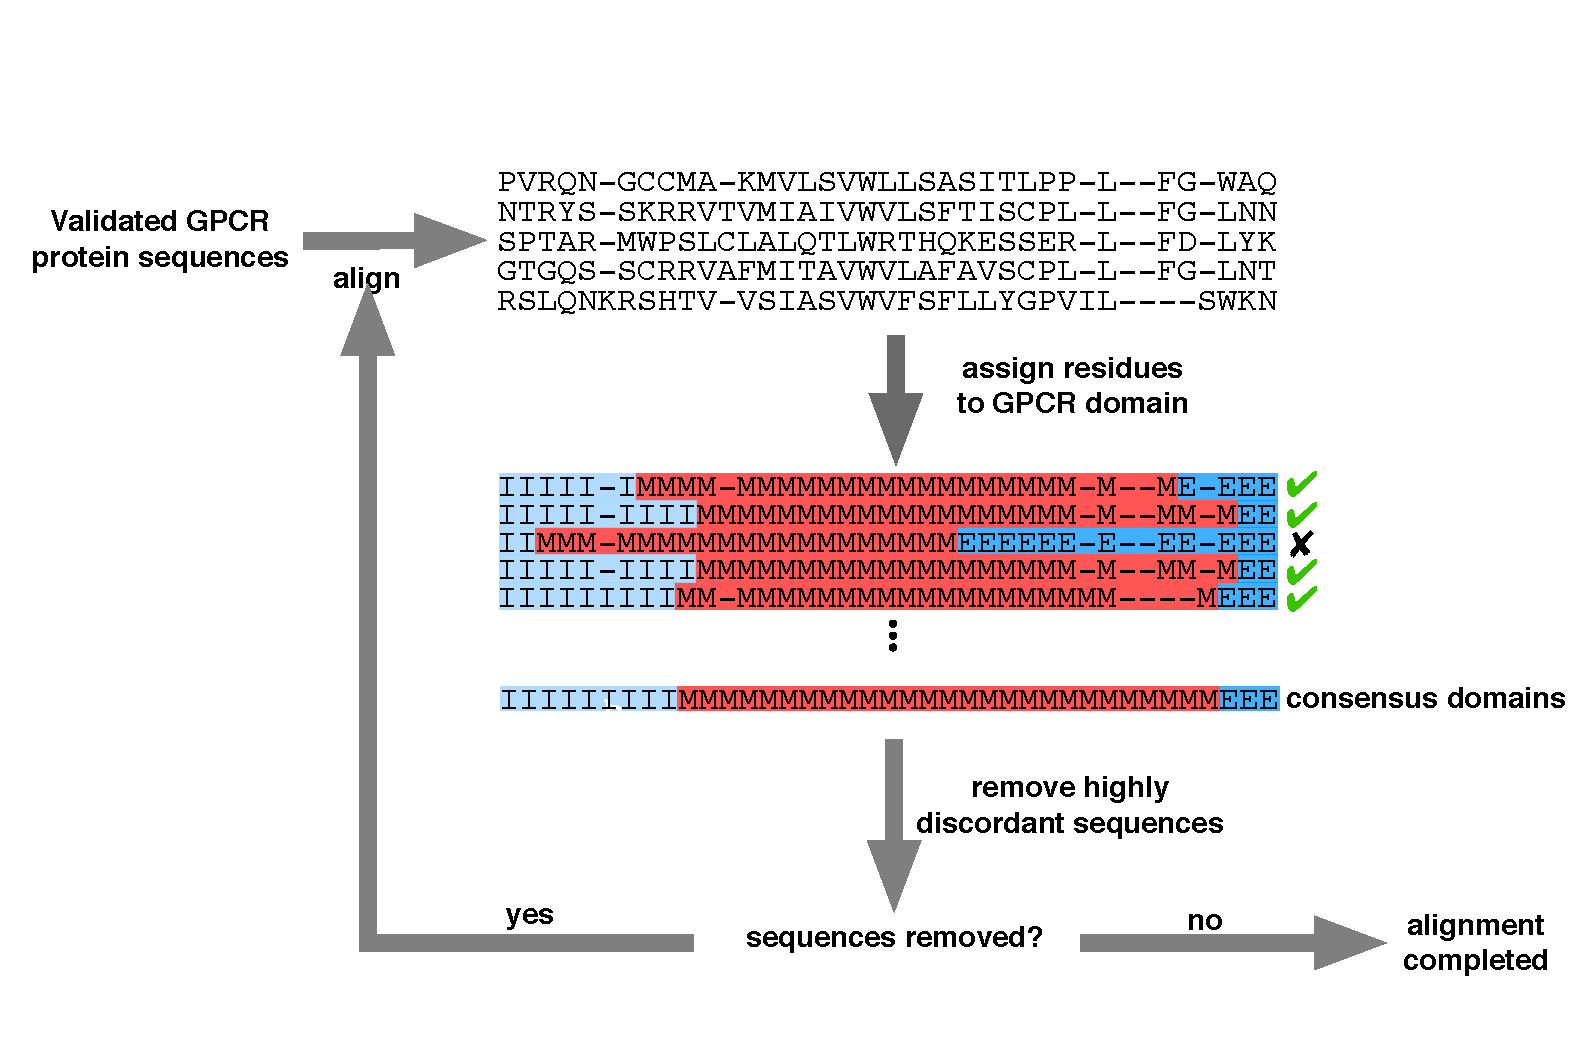
\includegraphics[width=18cm]{figures/alignment_flowchart.pdf}}
	\caption{\label{flowchart} Iterative alignment strategy to create a structurally-curated multiple sequence alignment. Starred sequence is consensus structure. I=inner, M=membrane, O=outer. Sequences were removed if $\geq 5\%$ of columns belonged to a different structural domain than the respective consensus domain.}
\end{figure}


\newpage


\begin{figure}[htbp]
	\centerline{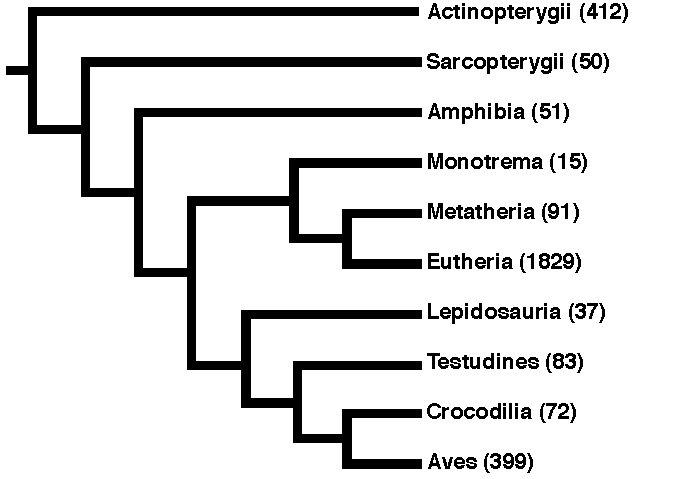
\includegraphics[width=7cm]{figures/taxonomic_distribution.pdf}}
	\caption{\label{taxa_dist} Cladogram of the taxonomic distribution of all sequences in the final structurally-curated alignment. All sequences were members of the \emph{Euteleostomi} clade of jawed vertebrates. Numbers in parentheses indicate the total number of biogenic amine receptors in the respective clade.}
\end{figure}

\vspace{3cm}

\begin{table}[htbp]
	\centering
	\begin{tabular}{l c l l c}
		\hline\noalign{\smallskip}
		\multicolumn{1}{c}{Alignment} & \multicolumn{1}{c}{Partitions?} & \multicolumn{1}{c}{$\ln L$} & \multicolumn{1}{c}{k} & \multicolumn{1}{l}{$\Delta$AIC} \\
		\hline\noalign{\smallskip}
		Structural Masked & Yes & -505500.8 & 6115 & 0 \\
		Structural Masked & No & -515991.7 & 6095 & 1752 \\  
		Structural Unmasked & Yes & -515343.6 & 6115 & 19685 \\
		Structural Unmasked & No & -515991.7 & 6095 & 20941 \\ 
		Naive & No &  -589703.7 & 6945 & 170047 \\
		\noalign{\smallskip}\hline\noalign{\smallskip} 
	\end{tabular}
	\caption{\label{tab:phylo_AIC} $\Delta$AIC scores relative to the best performing for phylogenies.  AIC is computed as AIC $= 2(k - \ln L)$, where $k$ is the number of free parameters of the model, and $\ln L$ is the log-likelihood \citep{Akaike1974,BurnhamAnderson2004}.}
\end{table}


\newpage

\begin{figure}[htbp]
	\centerline{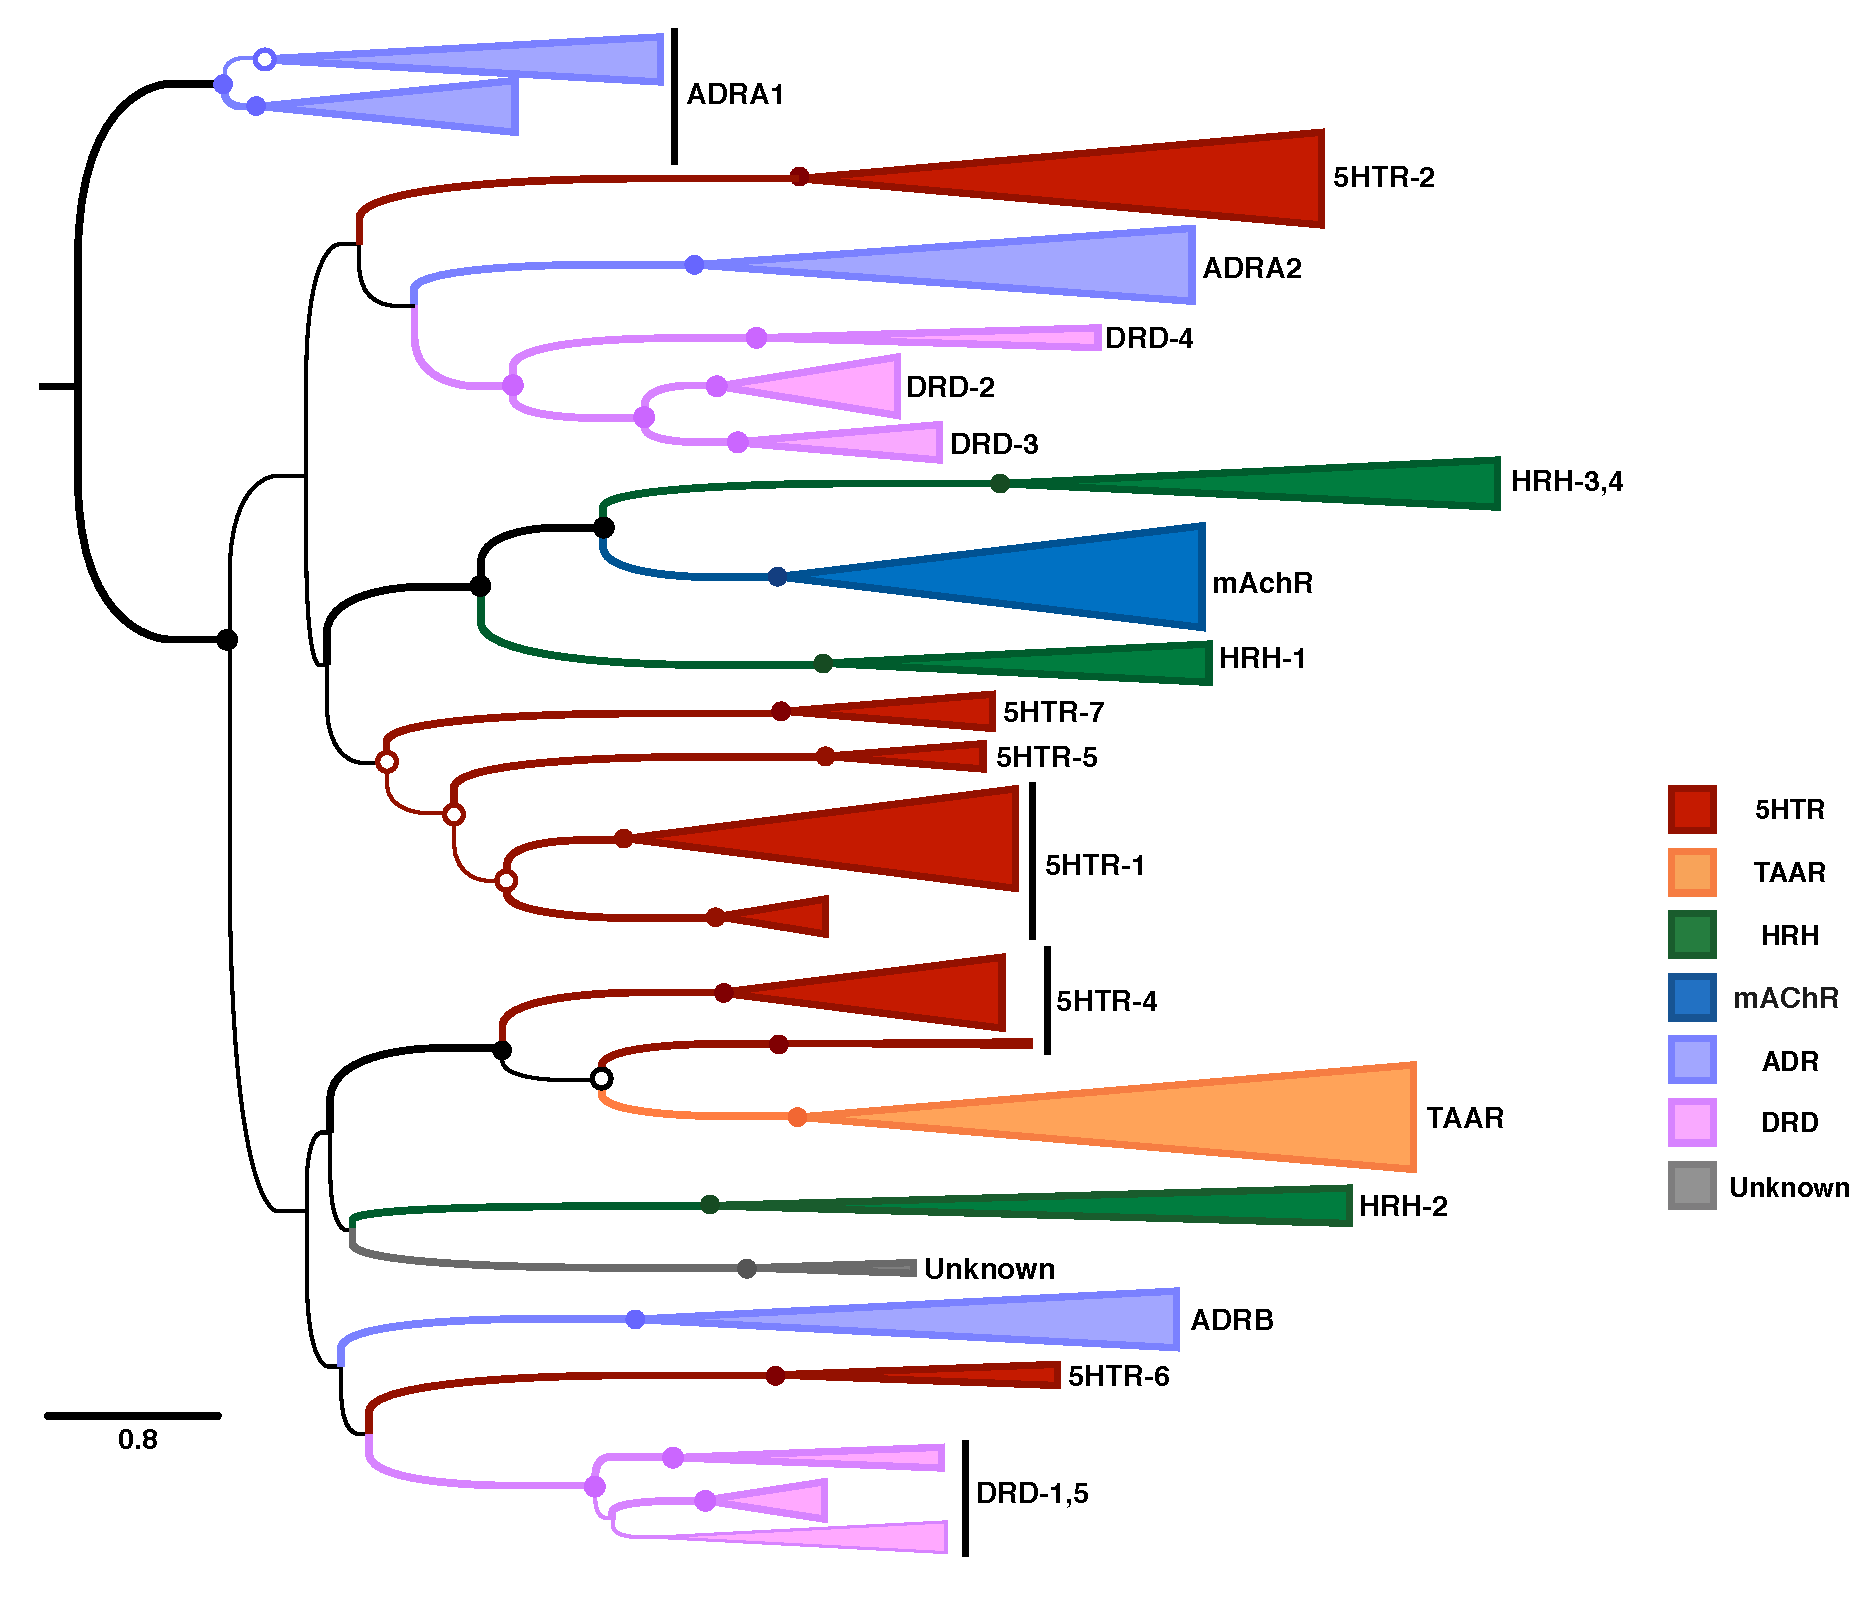
\includegraphics[width=18cm]{figures/masked_part_phylogeny.pdf}}
	\caption{\label{phylogeny} Maximum likelihood phylogeny of Vertebrate bioamine receptors built using the masked structural protein MSA alignment in RAxML. Nodes with open circles indicate $\geq 50\%$ bootstrap support, and nodes with closed circles and thick lines indicate $\geq 90\%$ bootstrap support. Bioaminergic receptors are abbreviated as 5HTR, serotonin receptors; TAAR, trace amine-associated receptors; HRH, histamine receptors; mAChr, muscarinic acetylcholine receptors; ADR, adreneric receptors; and DRD, dopamine receptors. The clade labeled ``Unknown'' could not be clearly identified as one of the major receptor types. Likely, this is a herp-specific gene...}
\end{figure}


\newpage

\begin{figure}[htbp]
	\centerline{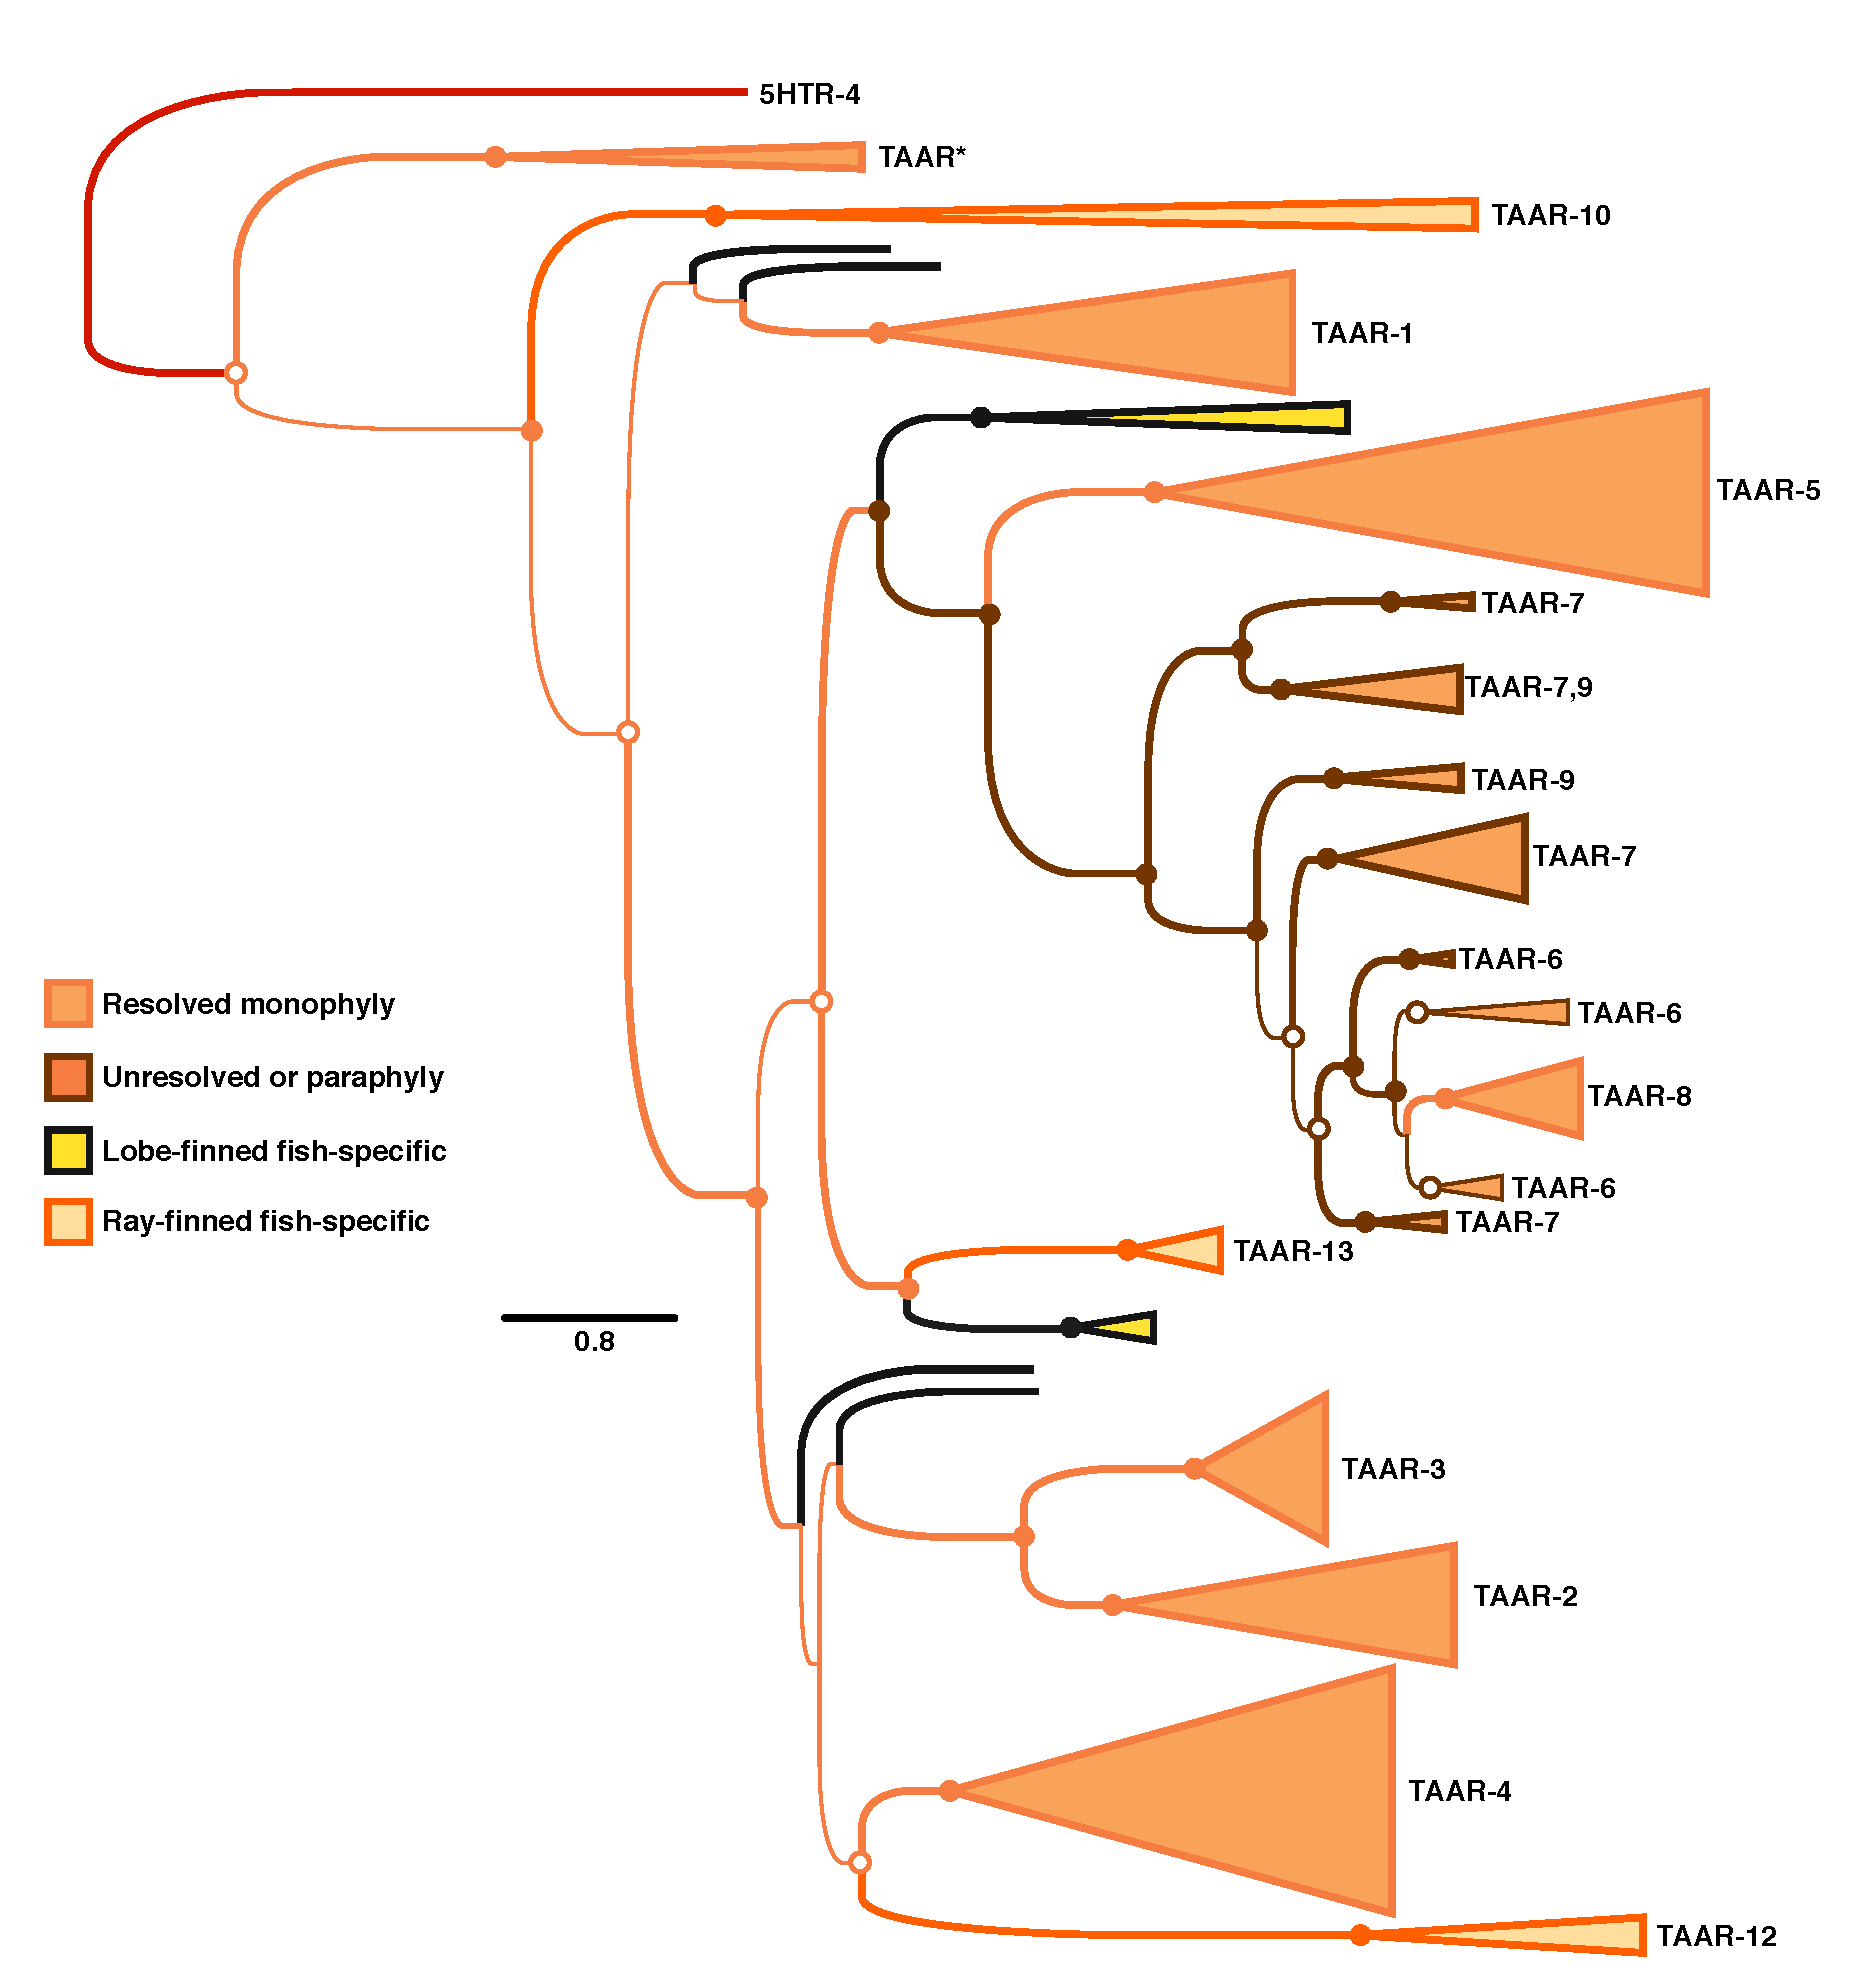
\includegraphics[width=15cm]{figures/taar_phylogeny.pdf}}
	\caption{\label{taar_tree} Specifically the TAAR clades from Figure~\ref{phylogeny}. We find neat coelocanth stuff!}
\end{figure}



\end{document}